\documentclass{beamer}\usepackage{knitr}
\usetheme{Singapore}

\usepackage{amsmath}
\usepackage{natbib}
\usepackage{hyperref}


\title{Sample Size Estimation}
\author{Lyron Winderbaum}













\IfFileExists{upquote.sty}{\usepackage{upquote}}{}
\begin{document}



\section{Intro}

\maketitle

\begin{frame}
  \frametitle{The Question}
  
  Diagnostic technology can distinguish between diseased (positive) and non-diseased (negative) blood samples.
  
  This technology has a sensitivity of at least 99\% and a specificity of at least 87\%.
  
  What is the minimum sample size needed to, with 90\% probability, obtain both:
  \begin{itemize}
    \item A point estimate for the sensitivity above 98\%, and
    \item The lower bound of a 95\% confidence interval above 96\%.
  \end{itemize}
  
\end{frame}



\section{Point Estimate}

\begin{frame}
  \frametitle{Notation}
  
  \begin{itemize}
    \item $n$: sample size
    \item $x$: number of true positives observed.
    \item $\hat{p}$: point estimate for sensitivity.
  \end{itemize}
  
\end{frame}



\begin{frame}
\frametitle{Approach}

The way I approached this was to:
\begin{itemize}
  \item Choose a method for calculating the point-estimate $\hat{p}$. 
  \item For all $n$ between 1 and 1000:
  \begin{itemize}
    \item Calculate $\hat{p}$ for every possible outcome $x$ between $0$ and $n$.
    \item For those that produce $\hat{p} > 0.98$, calculate and sum their binomial probabilities (assuming the true sensitivity is $0.99$).
  \end{itemize}
  \item Plot $n$ against the probability of satisfying the criteria $\hat{p} > 0.98$ to find the point at which the sample size is large enough that this probability is $> 90\%$. 
\end{itemize}

\end{frame}

\begin{frame}
\frametitle{Jeffreys Point Estimate}
I'll use the Jeffreys estimate:

\begin{equation*}
  \hat{p} = \frac{x + 0.5}{n + 1}
\end{equation*}

Which is the mean of the posterior distribution when a Jeffreys prior is used. It is also a compromise between the MLE and Laplace's Law of Succession (which is the mean of the posterior when using a uniform prior).

\end{frame}

% \begin{frame}
% \frametitle{MLE}
% <<plot_MLE_1, dependson=c('plotting', 'analysis'), fig.width=4.5, fig.height=3, out.width="\\linewidth">>=
% p = pest_plot(subset(df.pest, Estimate == "MLE"))
% print(p)
% @
% \end{frame}
% 
% \begin{frame}
% \frametitle{MLE}
% <<plot_MLE_2, dependson=c('plotting', 'analysis'), fig.width=4.5, fig.height=3, out.width="\\linewidth">>=
% p = pest_plot(subset(df.pest, Estimate == "MLE"))
% p = p + geom_line(data = subset(df.pest.low, Estimate == "MLE"))
% print(p)
% @
% \end{frame}
% 
% \begin{frame}
% \frametitle{MLE}
% <<plot_MLE_3, dependson=c('plotting', 'analysis'), fig.width=4.5, fig.height=3, out.width="\\linewidth">>=
% p = pest_plot(subset(df.pest, Estimate == "MLE" & n > 240 & n < 320))
% p = p + geom_line(data = subset(df.pest.low, Estimate == "MLE" & n > 240 & n < 320))
% print(p)
% @
% \end{frame}

% \subsection{Laplace's Law of Succession.}
% 
% \begin{frame}
% \frametitle{Laplace's Law of Succession.}
% <<plot_Laplace_1, dependson=c('plotting', 'analysis'), fig.width=4.5, fig.height=3, out.width="\\linewidth">>=
% p = pest_plot(subset(df.pest, Estimate == "Laplace"))
% print(p)
% @
% \end{frame}
% 
% \begin{frame}
% \frametitle{Laplace's Law of Succession.}
% <<plot_Laplace_2, dependson=c('plotting', 'analysis'), fig.width=4.5, fig.height=3, out.width="\\linewidth">>=
% p = pest_plot(subset(df.pest, Estimate == "Laplace"))
% p = p + geom_line(data = subset(df.pest.low, Estimate == "Laplace"))
% print(p)
% @
% \end{frame}
% 
% \begin{frame}
% \frametitle{Laplace's Law of Succession.}
% <<plot_Laplace_3, dependson=c('plotting', 'analysis'), fig.width=4.5, fig.height=3, out.width="\\linewidth">>=
% p = pest_plot(subset(df.pest, Estimate == "Laplace" & n > 240 & n < 480))
% p = p + geom_line(data = subset(df.pest.low, Estimate == "Laplace" & n > 240 & n < 480))
% print(p)
% @
% \end{frame}



\subsection{Jeffreys}

\begin{frame}
\frametitle{Jeffreys Point Estimate}
\begin{knitrout}
\definecolor{shadecolor}{rgb}{0.969, 0.969, 0.969}\color{fgcolor}

{\centering 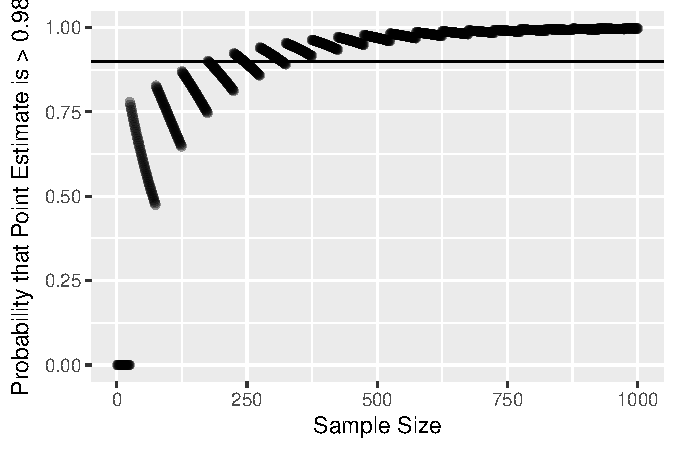
\includegraphics[width=\linewidth]{figure/plot_Jeffreys_1-1} 

}



\end{knitrout}
\end{frame}

\begin{frame}
\frametitle{Jeffreys Point Estimate}
\begin{knitrout}
\definecolor{shadecolor}{rgb}{0.969, 0.969, 0.969}\color{fgcolor}

{\centering 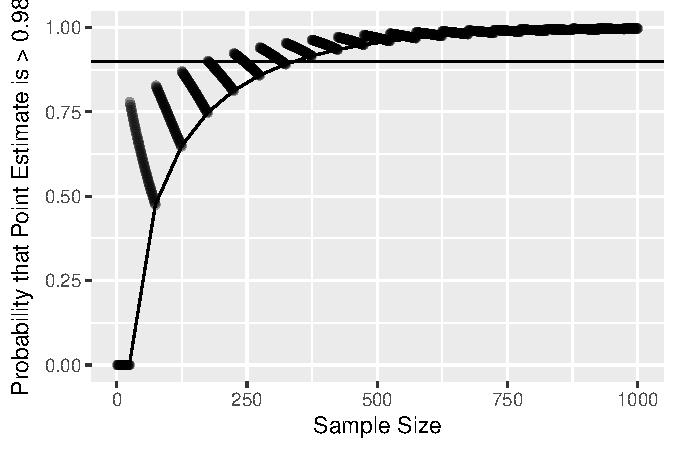
\includegraphics[width=\linewidth]{figure/plot_Jeffreys_2-1} 

}



\end{knitrout}
\end{frame}

\begin{frame}
\frametitle{Jeffreys Point Estimate}
\begin{knitrout}
\definecolor{shadecolor}{rgb}{0.969, 0.969, 0.969}\color{fgcolor}

{\centering 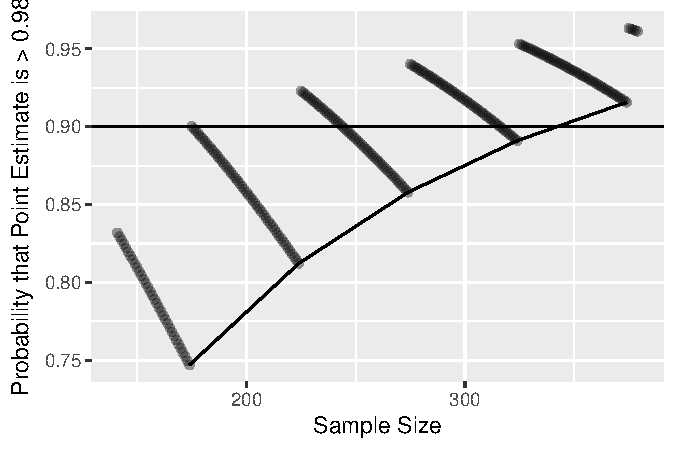
\includegraphics[width=\linewidth]{figure/plot_Jeffreys_3-1} 

}



\end{knitrout}
\end{frame}

\begin{frame}
\frametitle{Jeffreys Point Estimate}
\begin{knitrout}
\definecolor{shadecolor}{rgb}{0.969, 0.969, 0.969}\color{fgcolor}

{\centering 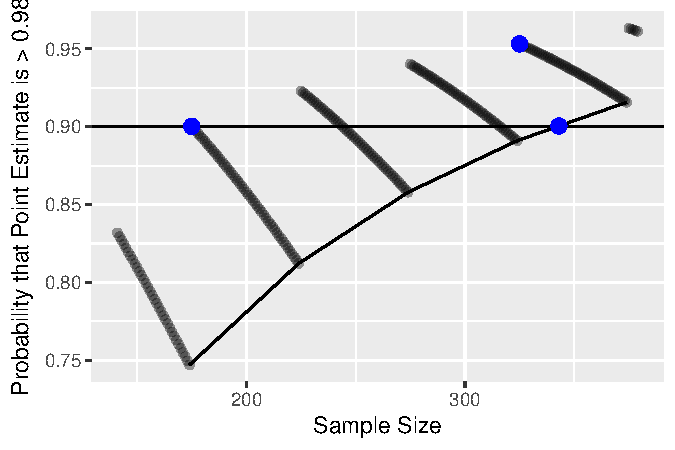
\includegraphics[width=\linewidth]{figure/plot_Jeffreys_4-1} 

}



\end{knitrout}
\end{frame}


\begin{frame}[fragile]
\frametitle{Jeffreys Point Estimate}

These three different approaches each give us a sample size estimate to varying degrees of conservativeness:

\begin{center}
  \begin{tabular}{ccc}
    First & Strict Min & Interpolation \\
    175 & 325 & 343 \\
  \end{tabular}
\end{center}

\end{frame}




% \begin{frame}
% \frametitle{Wilson}
% <<plot_Wilson_3, dependson=c('plotting', 'analysis'), fig.width=4.5, fig.height=3, out.width="\\linewidth">>=
% p = pest_plot(subset(df.pest, Estimate == "Wilson" & n > 340 & n < 580))
% p = p + geom_line(data = subset(df.pest.low, Estimate == "Wilson" & n > 340 & n < 580))
% print(p)
% @
% \end{frame}
% 
% \begin{frame}
% \frametitle{Bayes}
% <<plot_Bayes_3, dependson=c('plotting', 'analysis'), fig.width=4.5, fig.height=3, out.width="\\linewidth">>=
% p = pest_plot(subset(df.pest, Estimate == "Bayes" & n > 340 & n < 580))
% p = p + geom_line(data = subset(df.pest.low, Estimate == "Bayes" & n > 340 & n < 580))
% print(p)
% @
% \end{frame}





\section{Confidence Interval}

\begin{frame}
\frametitle{Clopper-Pearson Exact}

I'll use the Clopper-Pearson Exact confidence interval, which has lower bound $p_0$ as the solution to

\begin{equation*}
\sum_{k = x}^{n}{\binom{n}{k}p_0^k(1-p_0)^{n-k}} = \alpha / 2
\end{equation*}

where $\alpha$ is the required significance level, in this case $0.05$. This lower bound can neatly be calculated as the $\alpha/2$ quantile of a beta distribution with shape parameters $x$ and $n - x + 1$ (\cite{Agresti1998}).
\end{frame}

\begin{frame}
\frametitle{Clopper-Pearson Exact}
\begin{knitrout}
\definecolor{shadecolor}{rgb}{0.969, 0.969, 0.969}\color{fgcolor}

{\centering 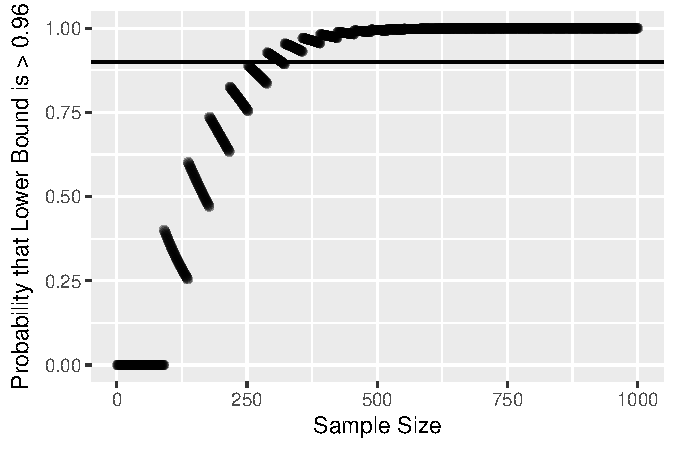
\includegraphics[width=\linewidth]{figure/plot_Exact_1-1} 

}



\end{knitrout}
\end{frame}

\begin{frame}
\frametitle{Clopper-Pearson Exact}
\begin{knitrout}
\definecolor{shadecolor}{rgb}{0.969, 0.969, 0.969}\color{fgcolor}

{\centering 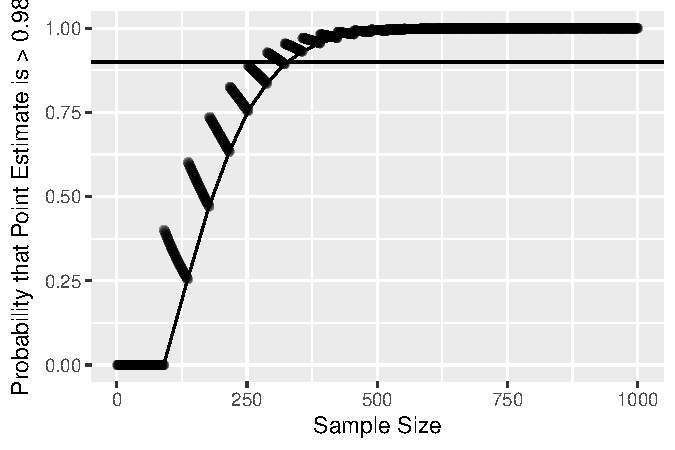
\includegraphics[width=\linewidth]{figure/plot_Exact_2-1} 

}



\end{knitrout}
\end{frame}

\begin{frame}
\frametitle{Clopper-Pearson Exact}
\begin{knitrout}
\definecolor{shadecolor}{rgb}{0.969, 0.969, 0.969}\color{fgcolor}

{\centering 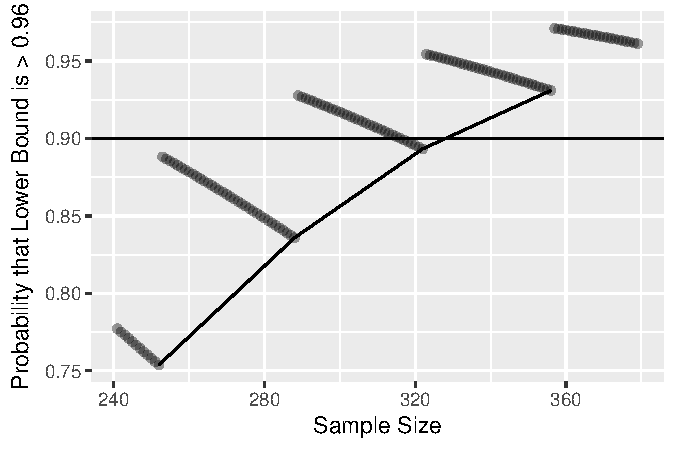
\includegraphics[width=\linewidth]{figure/plot_Exact_3-1} 

}



\end{knitrout}
\end{frame}

\begin{frame}
\frametitle{Clopper-Pearson Exact}
\begin{knitrout}
\definecolor{shadecolor}{rgb}{0.969, 0.969, 0.969}\color{fgcolor}

{\centering 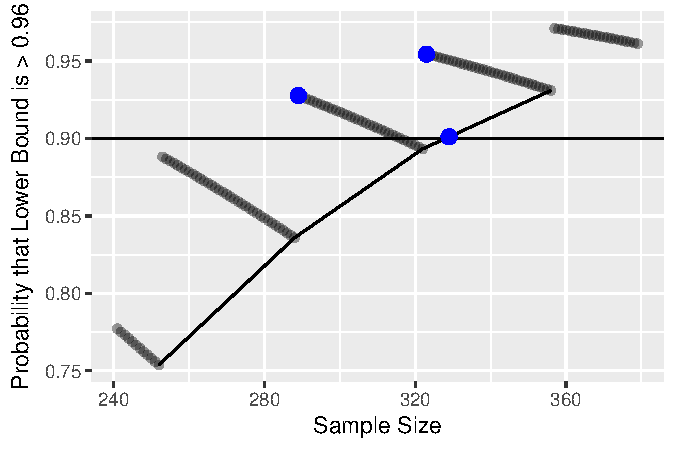
\includegraphics[width=\linewidth]{figure/plot_Exact_4-1} 

}



\end{knitrout}
\end{frame}




% \begin{frame}
% \frametitle{Adjusted Wald}
% <<plot_adjWald_1, dependson=c('plotting', 'analysis'), fig.width=4.5, fig.height=3, out.width="\\linewidth">>=
% p = conf_plot(subset(df.conf, Estimate == "adjWald"))
% print(p)
% @
% \end{frame}
% 
% \begin{frame}
% \frametitle{Adjusted Wald}
% <<plot_adjWald_2, dependson=c('plotting', 'analysis'), fig.width=4.5, fig.height=3, out.width="\\linewidth">>=
% p = pest_plot(subset(df.conf, Estimate == "adjWald"))
% p = p + geom_line(data = subset(df.conf.low, Estimate == "adjWald"))
% print(p)
% @
% \end{frame}
% 
% \begin{frame}
% \frametitle{Adjusted Wald}
% <<plot_adjWald_3, dependson=c('plotting', 'analysis'), fig.width=4.5, fig.height=3, out.width="\\linewidth">>=
% p = conf_plot(subset(df.conf, Estimate == "adjWald" & n > 240 & n < 480))
% p = p + geom_line(data = subset(df.conf.low, Estimate == "adjWald" & n > 240 & n < 480))
% print(p)
% @
% \end{frame}








\section{Discussion}


\begin{frame}[fragile]
\frametitle{Sample Size Reccomendation}

The sample size estimates for the point estimate criteria were:

\begin{center}
  \begin{tabular}{ccc}
    First & Strict Min & Interpolation \\
    175 & 325 & 343 \\
  \end{tabular}
\end{center}

and the equivalent estimates for the confidence interval criteria are:

\begin{center}
  \begin{tabular}{ccc}
    First & Strict Min & Interpolation \\
    289 & 323 & 329 \\
  \end{tabular}
\end{center}

Based on these calculations, the most conservative estimate would be $n = 343$, although I would still consider $n = 325$ quite reasonable and still quite conservative.

\end{frame}


\begin{frame}
  \frametitle{Assumptions}
  
  \begin{itemize}
    \item Results will be distributed according to a Binomial distribution.
    \item Cannot use prior knowledge about the sensitivity to inform our calculations.
  \end{itemize}
  
\end{frame}

\begin{frame}
  \frametitle{Additional Considerations}
  
  \begin{itemize}
    \item As is, these criteria could be manipulated:
      \begin{itemize}
        \item There is no criteria requiring a certain level of specificity.
        \item There is no criteria that prior knowledge cannot be used in calculation of confidence intervals and point estimates.
      \end{itemize}
    \item Knowledge about the cost per sample, and the consequences of failing to meet the criteria, could be used to optimise the choice of sample size.
  \end{itemize}
  
\end{frame}

\begin{frame}
{\Huge Questions?}
\end{frame}



\section{Appendices}


\subsection{Comments and other Point Estimates}

\begin{frame}
  \frametitle{Other Point Estimates}
  
  There are a number of different methods for point estimation:
  \begin{itemize}
    \item MLE: $\hat{p} = \frac{x}{n}$,
    \item Jeffreys: $\hat{p} = \frac{x + 0.5}{n + 1}$,
    \item Laplace: $\hat{p} = \frac{x + 1}{n + 2}$,
    \item Bayes: $\hat{p} = \frac{x + 2}{n + 4}$,
    \item Wilson: $\hat{p} = \frac{x + \frac{z^2}{2}}{n + z^2}$ (\cite{Wilson1927}),
    % Note: $z$ is the critical point from the standard normal distribution.
  \end{itemize}
  and more. \cite{Chew1971} offer a good review of point estimates for a binomial proportion.
  
\end{frame}



\begin{frame}[fragile]
\frametitle{Point Estimate Summary}
\begin{center}
  \begin{tabular}{lccc}
              & First & Strict Min & Interpolation \\
    MLE       & 1 & 251 & 266 \\
    Jeffreys  & 175 & 325 & 343 \\
    Laplace   & 299 & 399 & 414 \\
    Wilson    & 443 & 493 & 539 \\
    Bayes     & 447 & 547 & 549 \\
  \end{tabular}
\end{center}
\end{frame}


\subsection{Confidence Intervals}

\begin{frame}
  \frametitle{Confidence Intervals}
  
  There are many methods for confidence interval estimation as well, including:
  \begin{itemize}
    \item Exact (\cite{Clopper1934})
    \item Wilson Score (\cite{Wilson1927})
    \item Continuity-Corrected Wilson Score
    \item Wald
    \item Adjusted Wald (\cite{Agresti1998})
    \item Jeffreys
  \end{itemize}
  and more. \cite{Agresti1998} offer a good review of interval estimation methods for a binomial proportion.
  
\end{frame}


\begin{frame}[fragile]
\frametitle{Confidence Interval Summary}
\begin{center}
  \begin{tabular}{lccc}
              & First & Strict Min & Interpolation \\
    Exact     & 289 & 323 & 329 \\
    Wilson    & 288 & 323 & 329 \\
    cWilson   & 306 & 340 & 360 \\
    Agresti-Coull   & 297 & 331 & 343 \\
    Wald      & 1 & 197 & 223 \\
    adjWald   & 300 & 333 & 348 \\
    Jeffreys  & 235 & 271 & 297 \\
  \end{tabular}
\end{center}
\end{frame}

\subsection{Colophon}

\begin{frame}
\frametitle{Colophon}

These slides where written using \LaTeX in \href{http://www.rstudio.com/ide/}{Rstudio}. \href{http://yihui.name/knitr/}{knitr} was used to embed the R code that performed the analysis and generated the plots for this presentation. The complete source is available \href{https://github.com/Armadilloa16/LBT\_interview\_presentation}{my github}. This colophon was inspired by that in the book \href{http://r-pkgs.had.co.nz/intro.html\#intro-colophon}{R packages} by Hadley Wickham.

\end{frame}



\begin{frame}{Bibliography}
\bibliographystyle{plainnat}
\bibliography{references}
\end{frame}



\end{document}
